\documentclass{article}
\usepackage[bottom=2cm, right=1.5cm, left=1.5cm, top=2cm]{geometry}
\usepackage{amsmath}
\usepackage{amssymb}
\usepackage{amsthm}
\usepackage{enumitem}
\usepackage{exercise} % Exercises Style
\usepackage{graphicx}
\usepackage{caption}
\usepackage{environ}



% Enable Code
\usepackage{minted}
\let \extra T

\newcommand{\vect}[1]{\boldsymbol{#1}}
\DeclareMathOperator{\Tr}{Tr}
\DeclareMathOperator{\Cov}{Cov}
\DeclareMathOperator{\Var}{Var}
\DeclareMathOperator{\E}{E}

\usepackage{fancyhdr}
\newenvironment{solution}
  {\renewcommand\qedsymbol{$\blacksquare$}\begin{proof}[Solution]$ $}
  {\end{proof}}

\title{Solutions to Assignment 4}
\author{Rongfei Jin}
\begin{document}

\pagestyle{fancy}
\fancyhf{}%
\fancyhead[L]{\textbf{DS5220 \ Assignment 4}}
\fancyhead[R]{\textbf{Rongfei Jin}}
\fancyfoot[C]{\thepage}%
\maketitle

\section{Conceptual 1}

\begin{solution}
    \begin{align*}
        \frac{p(X)}{1-p(X)} & = \frac{\frac{e^{\beta_0 + \beta_1 X}}{1+e^{\beta_0 + \beta_1 X}}}{\frac{1+e^{\beta_0 + \beta_1 X}}{1+e^{\beta_0 + \beta_1 X}} - \frac{e^{\beta_0 + \beta_1 X}}{1+e^{\beta_0 + \beta_1 X}}} \\
                            & = \frac{e^{\beta_0 + \beta_1 X}}{1+e^{\beta_0 + \beta_1 X} - e^{\beta_0 + \beta_1 X}}                                                                                                       \\
                            & = e^{\beta_0 + \beta_1 X}
    \end{align*}
\end{solution}


\section{Conceptual 2}
\begin{solution}
    \begin{enumerate}[label=(\alph*)]
        \item
        \begin{align*}
            \Pr(Y = 1 | X_1 = 40, X_2 = 3.5) & = \frac{e^{\beta_0 + \beta_1 X_1 + \beta_2 X_2}}{1+e^{\beta_0 + \beta_1 X_1 + \beta_2 X_2}} \\
                                             & = \frac{e^{-6 + 0.05 \times 40 + 1 \times 3.5}}{1+e^{-6 + 0.05 \times 40 + 1 \times 3.5}}   \\
                                             & \approx 0.38
        \end{align*}

        \item
        \begin{align*}
            \frac{e^{\beta_0 + \beta_1 X_1 + \beta_2 X_2}}{1+e^{\beta_0 + \beta_1 X_1 + \beta_2 X_2}} &= 0.5 \\
             e^{\beta_0 + \beta_1 X_1 + \beta_2 X_2} &= 0.5 + 0.5 e^{\beta_0 + \beta_1 X_1 + \beta_2 X_2} \\
             e^{\beta_0 + \beta_1 X_1 + \beta_2 X_2} &= 1 \\
             \beta_0 + \beta_1 X_1 + \beta_2 X_2 &= 0 \\
             -6 + 0.05 \times X_1 + 3.5 & = 0 \\
             X_1 & = 50
        \end{align*}

    \end{enumerate}
\end{solution}
\newpage
\section{Applied 13(a-d)}
\begin{enumerate}[label=(\alph*)]
\item
\begin{figure}[h]
\centering
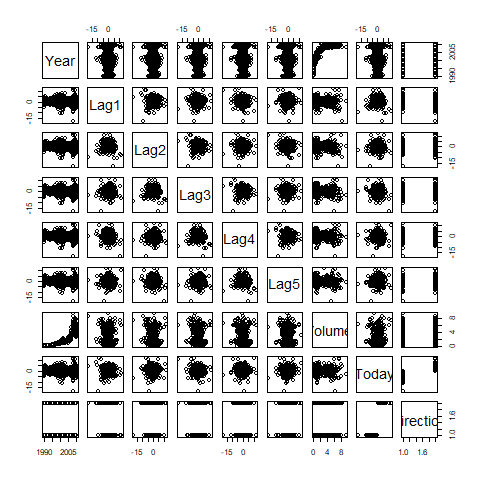
\includegraphics{pairs.png}
\caption{Pairs Plot}
\end{figure}
The Year and Volumne are strongly positively correlated with a correlation coefficient of 0.84. The Lags have extremly small correlations

\item Lag 2 is statistically significant
\item Confusion matrix tells the prediction correctly identify 54 Down and incorrectly identify 48 Up as Down. It correctly identify 557 Up and incorrectly identify 430 Down as Up. The number of false positive error is 430 and the number of false negative error is 48.

\item Accruacy 0.625 
\end{enumerate}
\newpage
\inputminted{r}{q13.R}
\newpage
\section{Applied 14(a-c, f)}
\begin{enumerate}[label=(\alph*)]
\item Shown in code below
\item Cylinder, Displacement, Horsepower and Weights are good predictors since there's less overlap between the two classes. The other predictors have more overlap between the two classes.
\item Shown in code below
\item[(f)] error rate is 0.09
\inputminted{r}{q14.R}
\end{enumerate}

\newpage
\section{Applied 16}
\inputminted{r}{q16.R}
Based on the logistic regression model, the nox, dis, rad, ptratio and medv are statistically significant predictors of crime rate where zn, chas have almost significant p-value. The nox, dis, rad, ptratio are positively correlated with crime rate while zn and chas are negatively correlated with crime rate. The model has an accuracy of 0.87.

\newpage
\section{Additional 1}
\begin{solution}
\begin{enumerate}[label=(\alph*)]
\item 
\[\frac{0}{1+e^x} < \frac{e^x}{1+e^x} < \frac{e^{x}}{e^{x}} \implies 0 < \frac{e^x}{1+e^x} <  1\]
\item
\begin{align*}
d(\frac{e^x}{1+e^x}) &= \frac{e^x(1+e^x) - e^x e^x}{(1+e^x)^2} \\
&= \frac{e^x}{(1+e^x)^2} \\
&= \frac{1}{1+e^x} \frac{e^x}{1+e^x} \\
&= \frac{1+e^x - e^x}{1+e^x} \frac{e^x}{1+e^x} \\
&= (1 - \frac{e^x}{1+e^x}) \frac{e^x}{1+e^x} \\
&= (1 - \phi(x)) \phi(x)
\end{align*}
\end{enumerate}
\end{solution}
\section{Additional 2}
\begin{solution}
\begin{align*}
\frac{d}{dp}(L(p|y)) &= -\frac{y}{p} + \frac{1-y}{1-p} \\
&= \frac{-y(1-p) + p - py}{p(1-p)} \\
&= \frac{-y + yp + p - py}{p(1-p)} \\
&= \frac{p - y}{p(1-p)} \\
\end{align*}
\end{solution}
\section{Additional 3}
\begin{solution}
\begin{align*}
\frac{d}{d\eta} l(\eta|y) &= -\frac{-y \phi'(\eta)}{\phi(\eta)} + \frac{(1-y)\phi'(\eta)}{1-\phi(\eta)} \\
&= -y[1-\phi(\eta)] + (1-y)\phi(\eta) \\
&= -y + \phi(\eta)
\end{align*}
\end{solution}
\newpage
\section{Additional 4}
\begin{solution}
    \begin{align*}
    \frac{\partial }{\partial \beta_0} l(\beta_0, \beta_1 | y, x) &= \frac{-y \phi'(\beta_0 + \beta_1 x)\cdot 1}{\phi(\beta_0 + \beta_1 x)} + \frac{(1-y)\phi'(\beta_0 + \beta_1 x)\cdot 1}{1-\phi(\beta_0 + \beta_1 x)} \\
    &= \phi(\beta_0 + \beta_1 x) - y
    \end{align*}

    \begin{align*}
    \frac{\partial }{\partial \beta_1} l(\beta_0, \beta_1 | y, x) &= \frac{-y \phi'(\beta_0 + \beta_1 x)\cdot x}{\phi(\beta_0 + \beta_1 x)} + \frac{(1-y)\phi'(\beta_0 + \beta_1 x)\cdot x}{1-\phi(\beta_0 + \beta_1 x)} \\
    &= -y[x-\phi(\beta_0 + \beta_1 x)\cdot x] + (1-y)\phi(\beta_0 + \beta_1 x)\cdot x \\
    &= (\phi(\beta_0 + \beta_1 x) - y)x
    \end{align*}
\end{solution}

\section{Additional 5}
\begin{solution}
\begin{align*}
\frac{\partial^2}{\partial \beta_0^2} l(\beta_0, \beta_1 | y, x) &= \frac{\partial}{\partial \beta_0} \frac{\partial}{\partial \beta_0} l(\beta_0, \beta_1 | y, x) \\
&= \frac{\partial}{\partial \beta_0} (\phi(\beta_0 + \beta_1 x) - y) \\
&= \phi'(\beta_0 + \beta_1 x) \\
&= \phi(\beta_0 + \beta_1 x)(1-\phi(\beta_0 + \beta_1 x))
\end{align*}

\begin{align*}
\frac{\partial}{\partial \beta_0 \partial \beta_1} l(\beta_0, \beta_1 | y, x) &= \frac{\partial}{\partial \beta_0} \frac{\partial}{\partial \beta_1} l(\beta_0, \beta_1 | y, x) \\
&= \frac{\partial}{\partial \beta_0} (\phi(\beta_0 + \beta_1 x) - y)x \\
&= \phi'(\beta_0 + \beta_1 x)x \\
&= x\phi(\beta_0 + \beta_1 x)(1-\phi(\beta_0 + \beta_1 x))
\end{align*}

\begin{align*}
\frac{\partial^2}{\partial \beta_1^2} l(\beta_0, \beta_1 | y, x) &= \frac{\partial}{\partial \beta_1} \frac{\partial}{\partial \beta_1} l(\beta_0, \beta_1 | y, x) \\
&= \frac{\partial}{\partial \beta_1} (\phi(\beta_0 + \beta_1 x) - y)x \\
&= (\phi'(\beta_0 + \beta_1 x)x - 0 ) \\
&= x^2\phi(\beta_0 + \beta_1 x)(1-\phi(\beta_0 + \beta_1 x))
\end{align*}

\end{solution}

\newpage
\section{Additional 6}
\begin{solution}
\begin{align*}
    \nabla \mathcal L (\beta | y, X) &= \begin{bmatrix}
    \frac{\partial}{\partial \beta_0} \mathcal L(\beta | y, X) \\
    \frac{\partial}{\partial \beta_1} \mathcal L(\beta | y, X) \\
    \end{bmatrix} \\
    &= \begin{bmatrix}
        \sum_{i=1}^{n} \frac{\partial}{\partial \beta_0} l(\beta | y_i, x_i) \\
        \sum_{i=1}^{n} \frac{\partial}{\partial \beta_1} l(\beta | y_i, x_i) \\
    \end{bmatrix} \\
    &= \sum_{i=1}^{n} \begin{bmatrix}
        \phi(\beta_0 + \beta_1 x_i) - y_i \\
        (\phi(\beta_0 + \beta_1 x_i) - y_i)x_i \\
    \end{bmatrix}
\end{align*}


\begin{align*}
    \nabla^2 \mathcal L (\beta | y, X) &= \begin{bmatrix}
    \frac{\partial^2}{\partial \beta_0^2} \mathcal L(\beta | y, X) &  \frac{\partial}{\partial \beta_0 \partial \beta_1} \mathcal L(\beta | y, X) \\
    \frac{\partial}{\partial \beta_0 \partial \beta_1} \mathcal L(\beta | y, X) & \frac{\partial^2}{\partial \beta_1^2} \mathcal L(\beta | y, X) \\
    \end{bmatrix} \\
    &= \begin{bmatrix}
        \sum_{i=1}^{n} \frac{\partial^2}{\partial \beta_0^2} l(\beta | y_i, x_i) & \sum_{i=1}^{n} \frac{\partial}{\partial \beta_0 \partial \beta_1} l(\beta | y_i, x_i) \\
        \sum_{i=1}^{n} \frac{\partial}{\partial \beta_0 \partial \beta_1} l(\beta | y_i, x_i) & \sum_{i=1}^{n} \frac{\partial^2}{\partial \beta_1^2} l(\beta | y_i, x_i) \\
    \end{bmatrix} \\
    &= \sum_{i=1}^{n} \begin{bmatrix}
        \phi(\beta_0 + \beta_1 x_i)(1-\phi(\beta_0 + \beta_1 x_i)) & x_i\phi(\beta_0 + \beta_1 x_i)(1-\phi(\beta_0 + \beta_1 x_i)) \\
        x_i\phi(\beta_0 + \beta_1 x_i)(1-\phi(\beta_0 + \beta_1 x_i)) & x_i^2\phi(\beta_0 + \beta_1 x_i)(1-\phi(\beta_0 + \beta_1 x_i)) \\
    \end{bmatrix} \\
    &= \sum_{i=1}^{n} \phi(\beta_0 + \beta_1 x_i)(1-\phi(\beta_0 + \beta_1 x_i)) \begin{bmatrix}
        1 & x_i \\
        x_i & x_i^2 \\
    \end{bmatrix}
\end{align*}
\end{solution}

\section{Additional 7}
The estimated beta values from newton's method is exactly the same as the beta values from glm function. 

\inputminted{r}{multiple-logistic-regression.R}



\end{document}